\documentclass[12pt,letterpaper,twoside]{article}

\newif\ifsolution\solutiontrue   % Include the solutions
%\newif\ifsolution\solutionfalse  % Exclude the solutions

\usepackage{cme213}
\usepackage{xcolor}
\usepackage{float}
\usepackage{graphicx}

\newcommand{\T}[1]{\text{\texttt{#1}}}
\newcommand{\V}[1]{\text{\textit{#1}}}

\begin{document}

{\centering \textbf{Preliminary Report: Neural Networks on CUDA\\}}
\vspace*{-8pt}\noindent\rule{\linewidth}{1pt}

Goal of the final project is to implement a neural network with parallel 
matrix-matrix operations across four GPUs. Our neural network will be used
to identify digits from hand-written images from the MNIST dataset.

\paragraph{Part 1: Accelerated Matrix Multiplication} Idea: parallelize generalized
inplace matrix mulitplication $C = \alpha*A*B + \beta*C$ across cores of one GPU. We 
will be able to use this to excute multiple steps in the neural network's feed forward 
and back propagation operations.

\begin{figure}[!htbp]
    \centering
    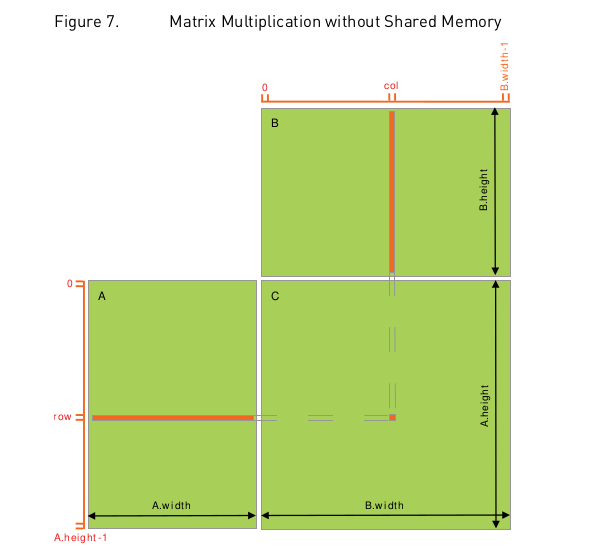
\includegraphics[scale=0.7]{gemm_naive.png}
    \caption{Naive matrix multiplication on GPU. Source: NVIDIA Programming Guide.}
\end{figure}

Our first implementation is correct but naive and inefficient. We ask each thread to 
compute a single value of the output matrix C. This requires each thread to read an 
entire row from matrix A and column from matrix B, resulting in a lot of repeated 
global memory accesses for the same information as we work our way through the 
multiplication. See code sample below.

\begin{cpp}
/* 
Routine to perform an in-place GEMM, i.e., C := alpha*A*B + beta*C
*/
__global__ 
void kernelGEMM(nn_real* __restrict__ A, nn_real* __restrict__ B, 
        nn_real* __restrict__ C, nn_real alpha, nn_real beta, 
            int M, int N, int K) 
{
    // Each thread computes one element of C
    // by accumulating results into Cvalue
    nn_real Cvalue = 0;
    int row = blockIdx.y * blockDim.y + threadIdx.y;
    int col = blockIdx.x * blockDim.x + threadIdx.x;

    if (row < M && col < N) 
    {
        for (int e = 0; e < K; ++e) 
        Cvalue += A[row + M*e] * B[e +  K*col];	
        
    C[row + col*M] = alpha*Cvalue + beta*C[row + col*M];
    }
}
\end{cpp}

\begin{verbatim}
Output from code
----------------

*** Grading mode 4 ***

main -g 4
Number of MPI processes = 1
Number of CUDA devices = 4

Entering GEMM Benchmarking mode! Stand by.

Starting GEMM 1: M = 3200; N = 4000; K = 3136
GEMM matched with reference successfully! Rel diff = 1.00042e-07
Time for reference GEMM implementation: 0.0710125 seconds
Time for my GEMM implementation: 3.04307 seconds
Completed GEMM 1

Starting GEMM 2: M = 3200; N = 400; K = 4000
GEMM matched with reference successfully! Rel diff = 4.57243e-07
Time for reference GEMM implementation: 0.00806695 seconds
Time for my GEMM implementation: 0.389439 seconds
Completed GEMM 2

Starting GEMM 3: M = 3200; N = 40; K = 4000
GEMM matched with reference successfully! Rel diff = 7.29707e-07
Time for reference GEMM implementation: 0.00140079 seconds
Time for my GEMM implementation: 0.0438419 seconds
Completed GEMM 3

*** Tests are complete ***
\end{verbatim}

In subsequent implementations we will try to improve the performance of this 
generalized matrix multiplication algorithm. For example, one speed-up would be
to make use of shared memory. To do this, we could have each thread block compute
a sub-matrix (of size matching thread block dimensions) in the output matrix, with
just the required blocks from A and B read into shared memory. This allows us to 
make use of increased access speed of shared memory and take advantage of a more
coalesced global memory access pattern.


\paragraph{Part 2: Parallelize Neural Network (Single GPU)} Idea: training a neural
network involves repeatedly updating weights and biases at each layer through forward
and backwards propagation. Internally, these operations are mostly various adaptations
of genralized matrix multiplication! We want to take existing sequential code and 
parallelize each using cuda code from part 1.

\begin{itemize}
    \item \textbf{Feed forward.} ...

    \item \textbf{Back propagation.} ...

    \item \textbf{Gradient descent.} ...
\end{itemize}

\begin{verbatim}
Starting at Sat May 28 01:16:51 UTC 2022
Running on hosts: icmet04
Running on 1 nodes.
Running on 4 processors.
Current working directory is /home/jelc/cme213-para/project

Output from code
----------------

* Mode 1 *
mpirun -np 1 /home/jelc/cme213-para/project/main -g 1
Number of MPI processes = 1
Number of CUDA devices = 4
num_neuron=100, reg=0.0001, learning_rate=0.0005, num_epochs=40, batch_size=800
Loading training data
Training data information:
Size of x_train, N =  60000
Size of label_train = 60000

Start Parallel Training
Time for Parallel Training: 7.85949 seconds
Precision on validation set for parallel training = 0.829167

Grading mode on. Now checking for correctness...

Max norm of diff b/w seq and par: W[0]: 1.54722e-07, b[0]: 5.94913e-07
l2  norm of diff b/w seq and par: W[0]: 1.90251e-07, b[0]: 5.54432e-07
Max norm of diff b/w seq and par: W[1]: 1.5259e-07, b[1]: 1.91096e-07
l2  norm of diff b/w seq and par: W[1]: 1.55346e-07, b[1]: 2.35015e-07

* Mode 2 *
mpirun -np 1 /home/jelc/cme213-para/project/main -g 2
Number of MPI processes = 1
Number of CUDA devices = 4
num_neuron=100, reg=0.0001, learning_rate=0.001, num_epochs=10, batch_size=800
Loading training data
Training data information:
Size of x_train, N =  60000
Size of label_train = 60000

Start Parallel Training
Time for Parallel Training: 2.24912 seconds
Precision on validation set for parallel training = 0.756

Grading mode on. Now checking for correctness...

Max norm of diff b/w seq and par: W[0]: 8.94932e-08, b[0]: 4.61505e-07
l2  norm of diff b/w seq and par: W[0]: 1.23037e-07, b[0]: 4.71446e-07
Max norm of diff b/w seq and par: W[1]: 1.46356e-07, b[1]: 4.07745e-07
l2  norm of diff b/w seq and par: W[1]: 1.54429e-07, b[1]: 3.5195e-07

* Mode 3 *
mpirun -np 1 /home/jelc/cme213-para/project/main -g 3
Number of MPI processes = 1
Number of CUDA devices = 4
num_neuron=100, reg=0.0001, learning_rate=0.002, num_epochs=1, batch_size=800
Loading training data
Training data information:
Size of x_train, N =  60000
Size of label_train = 60000

Start Parallel Training
Time for Parallel Training: 0.56508 seconds
Precision on validation set for parallel training = 0.463667

Grading mode on. Now checking for correctness...

Max norm of diff b/w seq and par: W[0]: 3.62044e-08, b[0]: 4.51159e-07
l2  norm of diff b/w seq and par: W[0]: 5.70983e-08, b[0]: 3.23318e-07
Max norm of diff b/w seq and par: W[1]: 6.22334e-08, b[1]: 2.59939e-07
l2  norm of diff b/w seq and par: W[1]: 7.5405e-08, b[1]: 1.77756e-07

*** Summary ***

2400           1.40465e-07    1.45118e-07    6.03892e-07    1.9369e-07     1.75842e-07    1.51356e-07    5.24816e-07    2.36566e-07    
600            8.31383e-08    1.35914e-07    6.12333e-07    3.84295e-07    1.13652e-07    1.48703e-07    4.68868e-07    3.25847e-07    
60             3.33698e-08    6.31382e-08    4.08258e-07    2.66437e-07    5.36129e-08    7.22897e-08    3.02703e-07    1.9781e-07     

\end{verbatim}

\textbf{Remarks on debgugging.} This step required significant debugging effort given 
the inherent complexity of indexing many different variations of parallel matrix 
operations. My approach here was to add \texttt{#if} and \texttt{#endif} statements 
after each major step of the sequential algorithm and try to reproduce that step using 
my parallel code. To test whether the two implementations matched, I re-used existing 
\texttt{checkErrors} and \textt{checkNNErrors} from the provided starter code test suite.


\paragraph{Part 3: Parallelize Training Batches (Multiple GPUs)} Idea: while each epoch 
needs to be executed sequentially, we can perform forwards and backwards propagation on 
batches within each epoch independently (and therefore in parallel). Our code from part 
2 should already make good use of hardware resources on a single GPU, however, in this 
project we have access to multiple GPUs! We use MPI to help coordinate sending different
training batches to different GPUs as well as receiving back and aggregating outputs from
each batch.

...
...

\begin{cpp}
    ...
    ...
\end{cpp}


\paragraph{Part 4: Profiling Parallel Code} Idea: use NVIDIA's Insight and Compute Systems
tool to interrogate performance of code and assess how to improve.

Insert profile screenshots ...
... something about focusing on arithmetic intensity
... also latency bound vs memory bound vs compute bound


Ideas to improve performance:
\begin{itemize}
    \item \textbf{Matrix multiplication.} ...

    \item \textbf{Kernel usage.} ...

    \item \textbf{Batching logic.} ... 

\end{itemize}

\end{document}
